\chapter{Conception fonctionnelle et technique}

\section{Introduction}

Dans ce chapitre, nous présentons la solution conceptuelle proposée pour la conception
du système \textbf{FinPulse}, une plateforme d'analyse d'investissement intelligente basée
sur l'intelligence artificielle. Cette solution vise à fournir aux investisseurs un outil
fiable pour évaluer la cohérence entre le discours marketing des entreprises et leur
réalité réglementaire, tout en assurant une flexibilité, une maintenabilité et une
évolutivité du système.

Ce chapitre répond à la question : \textit{comment concevoir le système ?} Pour cela,
nous aborderons successivement les contraintes du projet, les besoins fonctionnels et
non fonctionnels, avant d'introduire les choix architecturaux et technologiques qui
guideront l'implémentation.

\section{Objectifs et contraintes du projet}

La conception du système doit répondre à plusieurs contraintes techniques,
fonctionnelles et organisationnelles :

\begin{itemize}
    \item \textbf{Fiabilité des données} : Les analyses doivent reposer sur des sources
    réglementaires officielles (rapports 10-K déposés sur \textit{sec.gov}), garantissant
    ainsi l'exactitude et la traçabilité de l'information financière ;

    \item \textbf{Performance temps réel} : La Watchlist doit se mettre à jour en continu
    via un flux SSE (\textit{Server-Sent Events}) sans rechargement de page, afin
    d'offrir une expérience utilisateur fluide ;

    \item \textbf{Scalabilité} : L'architecture doit supporter l'ingestion régulière de
    nouveaux rapports SEC et l'ajout de nouvelles entreprises sans dégradation des
    performances ;

    \item \textbf{Sécurité} : Gestion des profils utilisateurs (Investisseur Prudent vs
    Spéculateur) avec authentification sécurisée et personnalisation des poids du score
    NCI ;

    \item \textbf{Interopérabilité} : Intégration avec des API externes (Alpha Vantage /
    Polygon.io pour les cours boursiers, NewsAPI / Yahoo Finance pour l'actualité
    financière) ;

    \item \textbf{Cohérence des données} : Utilisation de PostgreSQL avec l'extension
    PGVector pour centraliser à la fois les données structurées (scores, stratégies) et
    les embeddings vectoriels (chunks des rapports 10-K).
\end{itemize}

\section{Analyse des besoins}

\subsection{Besoins fonctionnels}

Les fonctionnalités essentielles identifiées s'organisent autour de trois grandes 
fonctionnalités de la plateforme.

\subsubsection{Fonctionnalité 1 — Chatbot d’analyse (Agent d’investissement et moteur de stratégie)}

\begin{itemize}
    \item \textbf{Agent d’investissement } : L’utilisateur soumet une idée 
    d’investissement en langage naturel (exemple : « Je souhaite investir dans Tesla 
    car la demande de véhicules électriques augmente »). Le système décompose l’idée, 
    interroge la base vectorielle par l’intermédiaire du mécanisme RAG, calcule le 
    score de cohérence $F_{consistency}$ et répond en citant les sections pertinentes 
    du rapport 10-K.

    \item \textbf{Moteur de stratégie } : L’utilisateur décrit sa stratégie 
    complète (secteur, horizon temporel, raisonnement). Le système génère un rapport 
    structuré en trois volets — preuves à l’appui, contradictions détectées dans les 
    documents SEC, précédents historiques — exporté au format PDF via un 
    \texttt{BeanOutputConverter} de Spring AI.

    \item \textbf{Analyse d’intention} : Le chatbot identifie automatiquement si 
    l’utilisateur sollicite le mode 1:1 (discussion interactive) ou le mode 1:2 
    (génération d’un rapport formel).

    \item \textbf{Score NCI personnalisé} : En mode 1:2, le système ajuste 
    dynamiquement le NCI global de l’entreprise en lui appliquant un malus 
    $F_{consistency}$ calculé à partir des arguments de l’utilisateur, produisant 
    ainsi un score de risque contextualisé.
\end{itemize}

\subsubsection{Fonctionnalité 2 — Surveillance automatisée}

\begin{itemize}
    \item \textbf{Sauvegarde de stratégie} : L’utilisateur peut enregistrer une 
    stratégie analysée. Le système active alors une surveillance continue sur 
    l’entreprise ciblée.

    \item \textbf{Détection de changements significatifs} : Une tâche planifiée 
    (\texttt{@Scheduled}) recalcule périodiquement le NCI global. Si la variation 
    dépasse un seuil configurable ($\Delta NCI > +15$ points) ou si de nouveaux 
    mots-clés critiques (risques) apparaissent, une alerte est déclenchée.

    \item \textbf{Notification multicanal} : Les alertes sont affichées dans la 
    plateforme et envoyées par courriel ou message à tous les utilisateurs ayant une 
    stratégie active sur l’entreprise concernée.
\end{itemize}

\subsubsection{Fonctionnalité 3 — Watchlist en temps réel}

\begin{itemize}
    \item \textbf{Épinglage d’entreprises} : L’utilisateur peut ajouter un nombre 
    illimité d’entreprises à sa watchlist.

    \item \textbf{Flux SSE en direct} : Pour chaque entreprise épinglée, la 
    plateforme diffuse en continu les informations suivantes :
    \begin{itemize}
        \item Score NCI actuel avec delta de tendance (indicateur vert, orange ou rouge) ;
        \item Variations des cours boursiers ($P_t$ vs $P_{t-24h}$) via Alpha Vantage 
        ou Polygon.io ;
        \item Jauge de \textit{sentiment shift} (divergence entre le discours du 
        10‑K et les actualités récentes) ;
        \item Actualités filtrées par IA, ne retenant que celles liées aux risques 
        identifiés dans le rapport 10‑K ;
        \item Archive de cohérence (graphique historique : axe des temps / axe des 
        scores NCI).
    \end{itemize}

    \item \textbf{Navigation contextuelle} : Chaque carte de la watchlist intègre des 
    boutons de redirection vers l’agent d’investissement, le tableau de bord détaillé 
    et l’archive de cohérence.
\end{itemize}

\subsubsection{Pipeline d’ingestion (socle commun)}

\begin{itemize}
    \item \textbf{Extraction SEC} : Un script Spring Boot récupère automatiquement 
    les derniers rapports 10‑K depuis \textit{sec.gov}.
    \item \textbf{Analyse sémantique} : Extraction des sections clés — 
    \textit{Item 1A} (Risques) et \textit{Item 7} (MD\&A).
    \item \textbf{Vectorisation} : Spring AI transforme les segments textuels 
    (chunks) en vecteurs de 1536 dimensions stockés dans la table 
    \texttt{documents\_embeddings} (PGVector).
    \item \textbf{Calcul du NCI global} : Batch nocturne mettant à jour les scores 
    de toutes les entreprises en base de données.
\end{itemize}

\subsection{Besoins non fonctionnels}

Ces besoins définissent les caractéristiques qualitatives du système.

\begin{itemize}
    \item \textbf{Performance} : Le pipeline d’ingestion doit s’exécuter en tâche de 
    fond sans dégrader la réactivité de l’interface utilisateur. Les requêtes de 
    similarité vectorielle doivent retourner leurs résultats dans un délai acceptable 
    pour le chatbot.

    \item \textbf{Maintenabilité} : L’architecture en microservices logiques 
    (P1 — Data Engine, P2 — RAG Developer, P3 — Sentinel, P4 — Fullstack) favorise 
    l’isolation des responsabilités et facilite les évolutions indépendantes de 
    chaque composant.

    \item \textbf{Disponibilité} : Le système de surveillance (fonctionnalité 2) doit 
    fonctionner en continu, y compris en dehors des plages horaires d’utilisation 
    active de la plateforme.

    \item \textbf{Extensibilité} : L’architecture doit permettre l’ajout de nouvelles 
    sources de données (autres types de documents SEC, nouvelles API de marché) sans 
    réécriture majeure.

    \item \textbf{Sécurité} : Les données des stratégies utilisateur sont sensibles. 
    L’accès doit être protégé par une authentification, et les communications avec 
    les API externes doivent être sécurisées.

    \item \textbf{Précision analytique} : Le score NCI doit refléter fidèlement la 
    divergence entre le discours marketing et la réalité réglementaire. Les 
    instructions (\textit{prompts}) du modèle de langage doivent être conçues pour 
    minimiser les hallucinations et maximiser la traçabilité des sources citées.
\end{itemize}
\section{Modélisation UML}
Pour modéliser la structure et les interactions du système, nous avons utilisé la méthode UML (\textit{Unified Modeling Language}), standard en ingénierie logicielle. \vspace{3mm}  \\Trois types de diagrammes ont été réalisés :\vspace{3mm}\\le \textbf{diagramme de cas d’utilisation}, qui décrit les fonctionnalités attendues du système du point de vue de l’utilisateur ; \\le \textbf{diagramme de classes}, qui représente les entités métier et leurs relations ; \\ les \textbf{diagrammes de séquences}, qui illustrent la chronologie des échanges entre les différents composants pour plusieurs scénarios clés.
\subsection{Diagramme de cas d'utilisation}
Afin de comprendre comment les différents acteurs interagiront avec la plateforme FinPulse, on a modélisé les exigences fonctionnelles à l'aide d'un diagramme de cas d'utilisation (figure 1). Cette étape de conception logicielle permet de visualiser les grandes fonctionnalités offertes par l'application, telles que l'analyse assistée par IA et la gestion des données financières, tout en précisant les conditions d'accès pour chaque profil d'utilisateur.
\subsubsection{Acteurs identifiés}
Le système \textbf{FinPulse} fait intervenir quatre acteurs principaux, chacun ayant des responsabilités et des droits d'accès spécifiques :

\begin{description}
    \item[Visiteur] : Il représente tout utilisateur non authentifié. Ses actions sont limitées à la création d'un compte ou à l'exploitation basique des données d'entreprises publiques.
    
    \item[Utilisateur] : C'est l'acteur principal authentifié. Il bénéficie de l'ensemble des services avancés : conversation avec l'assistant IA, demande et sauvegarde de rapports de stratégie, gestion de ses entreprises favorites et réception d'alertes personnalisées.
    
    \item[Assistant] : Cet acteur (système ou humain) intervient spécifiquement pour répondre aux requêtes de l'utilisateur lors de la récupération des données d'entreprise et du support à la décision.
    
    \item[Service d'ingestion de données (Acteur système)] : Acteur externe automatisé chargé d'alimenter la plateforme en données fraîches. Il est sollicité lors de la phase d'authentification et pour fournir les flux nécessaires à l'analyse financière.
\end{description}
\begin{figure}[H]
    \centering
    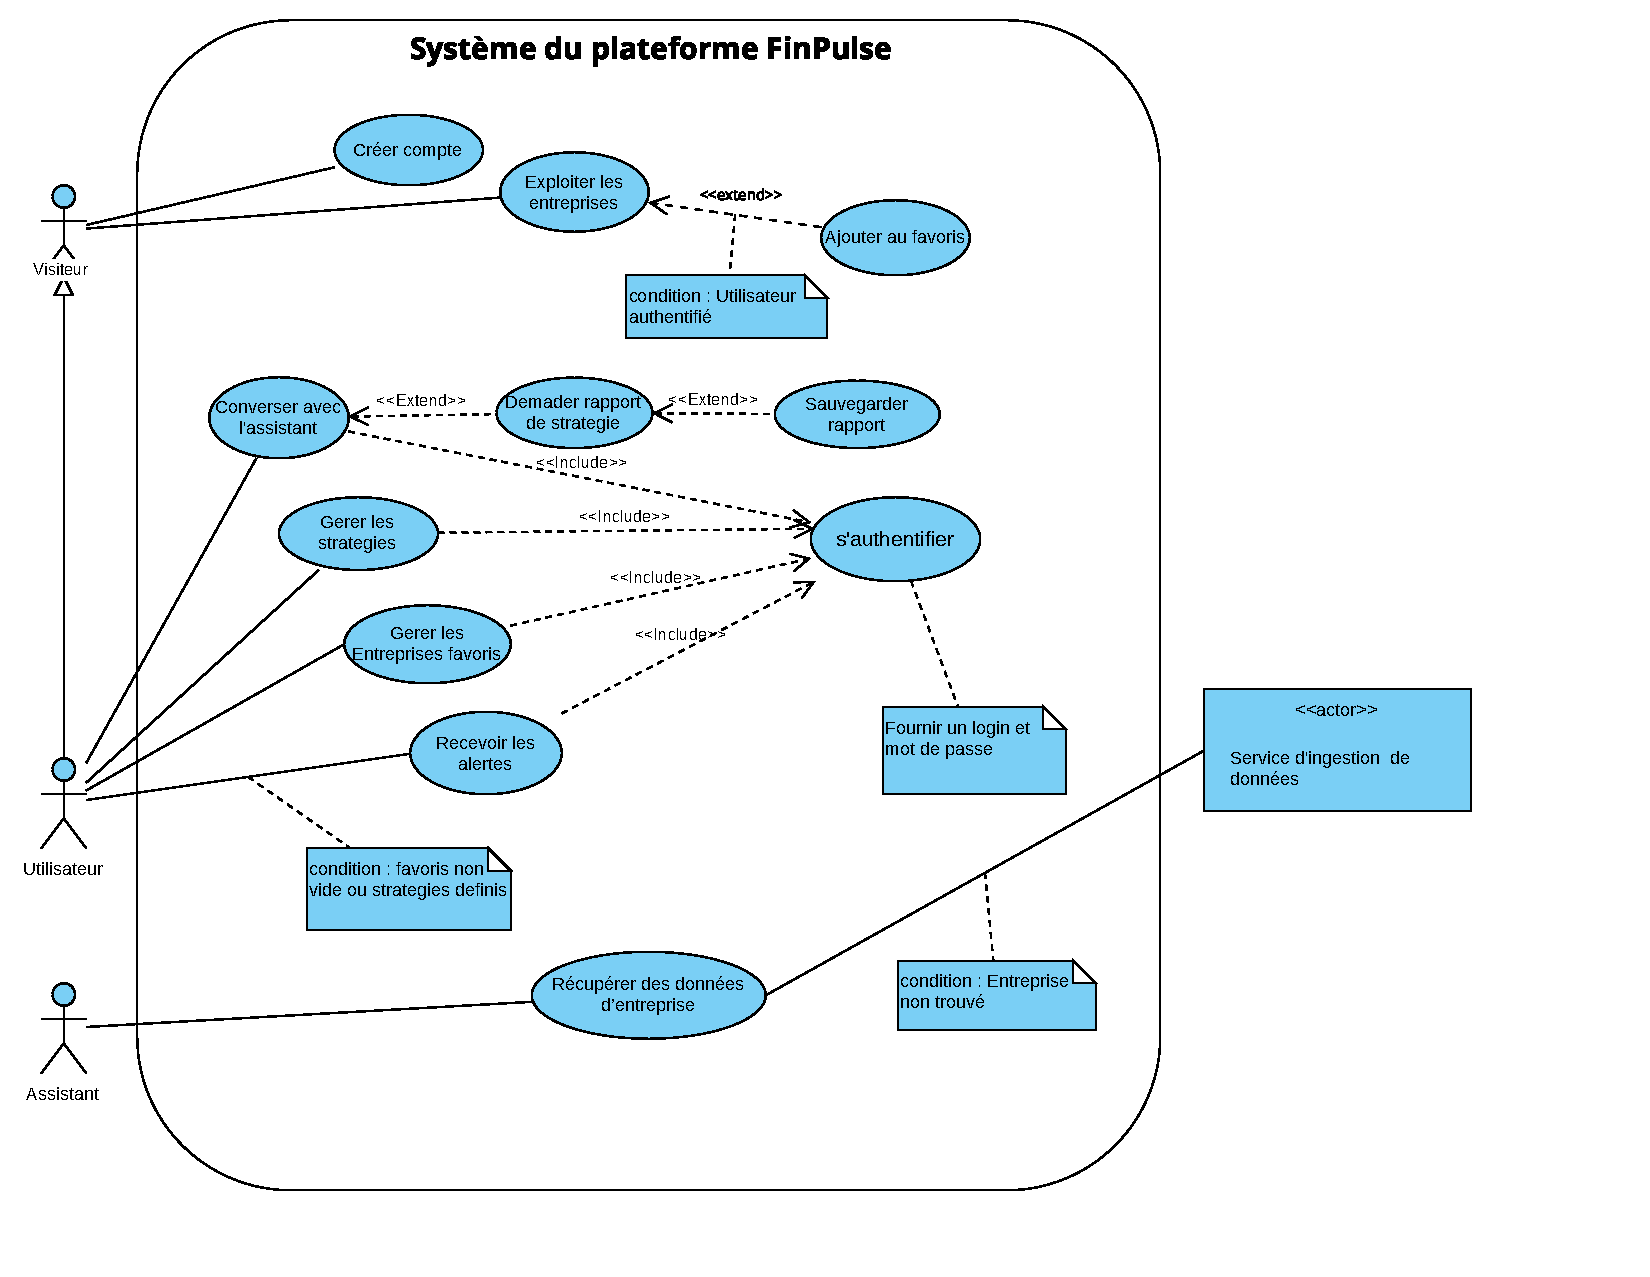
\includegraphics[width=1\linewidth]{images/usecase_finpulse.pdf}
    \caption{Diagramme de cas d'utilisation}
    \label{fig:usecase-finpulse}
\end{figure}
\subsection{Diagramme de classes}
\label{sec:class-diagram}

Le diagramme de classes (figure~\ref{fig:class}) représente la structure statique du système. Il identifie les principales entités, leurs attributs, méthodes (le cas échéant) ainsi que les relations entre elles (héritage, associations, compositions, agrégations). Cette modélisation constitue le socle du modèle de données et des services métier.

\subsubsection*{Entités principales du domaine}

Les classes peuvent être regroupées en plusieurs sous-ensembles fonctionnels :

\paragraph{1. Gestion des utilisateurs et des favoris}
Les classes \texttt{User}, \texttt{FavoriteCompany} et \texttt{FavoriteStrategy} gèrent les profils utilisateurs, leurs sociétés favorites et leurs stratégies personnalisées (indice NCI personnalisé). Un \texttt{User} possède une liste de \texttt{FavoriteCompany} (composition) et peut avoir plusieurs \texttt{FavoriteStrategy}.

\paragraph{2. Interaction et assistance (chat)}
Les classes \texttt{ChatSession} et \texttt{ChatMessage} modélisent les conversations. Une session (\texttt{ChatSession}) est associée à un utilisateur et à un contexte (ex. ticker d’une entreprise, type de contexte). Chaque message (\texttt{ChatMessage}) appartient à une session (relation non explicite dans le texte mais implicite via les attributs \texttt{companyTicker} et \texttt{contextType}).

\paragraph{3. Données financières fondamentales}
\vspace{-0.2cm}
\begin{itemize}
    \item \texttt{Companies} : société cotée (CIK, ticker, secteur, dates de dépôt).
    \item \texttt{Filing} et \texttt{FilingSection} : dépôts réglementaires (10-K, 10-Q, etc.) et leurs sections textuelles.
    \item \texttt{MarketPrice} : série temporelle des prix (ouverture, clôture, volume).
    \item \texttt{XBRLFact} : faits financiers structurés (concept, valeur, période, fiscal year/quarter).
    \item \texttt{InsiderTransaction} : transactions des initiés (dirigeants, administrateurs).
\end{itemize}

\paragraph{4. Indices et scores d’intelligence artificielle}
\vspace{-0.2cm}
\begin{itemize}
    \item \texttt{NCIScore} : score de confiance global (NCI global, bornes inf/sup, signaux textuel, fondamental, insider, anomalie) avec métadonnées (confiance, taux de couverture, événement).
    \item \texttt{SignalScore} : signaux multifactoriels (RKDS, GCE, ITA, convergence).
    \item \texttt{Embeddings} : représentations vectorielles (1024 dimensions) des sections de documents, avec scores de reconstruction et d’anomalie.
\end{itemize}

\paragraph{5. Services d’accès aux données}
Les classes \texttt{GetTimeSeriesConcept} et \texttt{GetXBRLFact} semblent être des artefacts de conception (repositories ou services) pour récupérer des séries temporelles et des faits XBRL.

\begin{figure}[H]
    \centering
    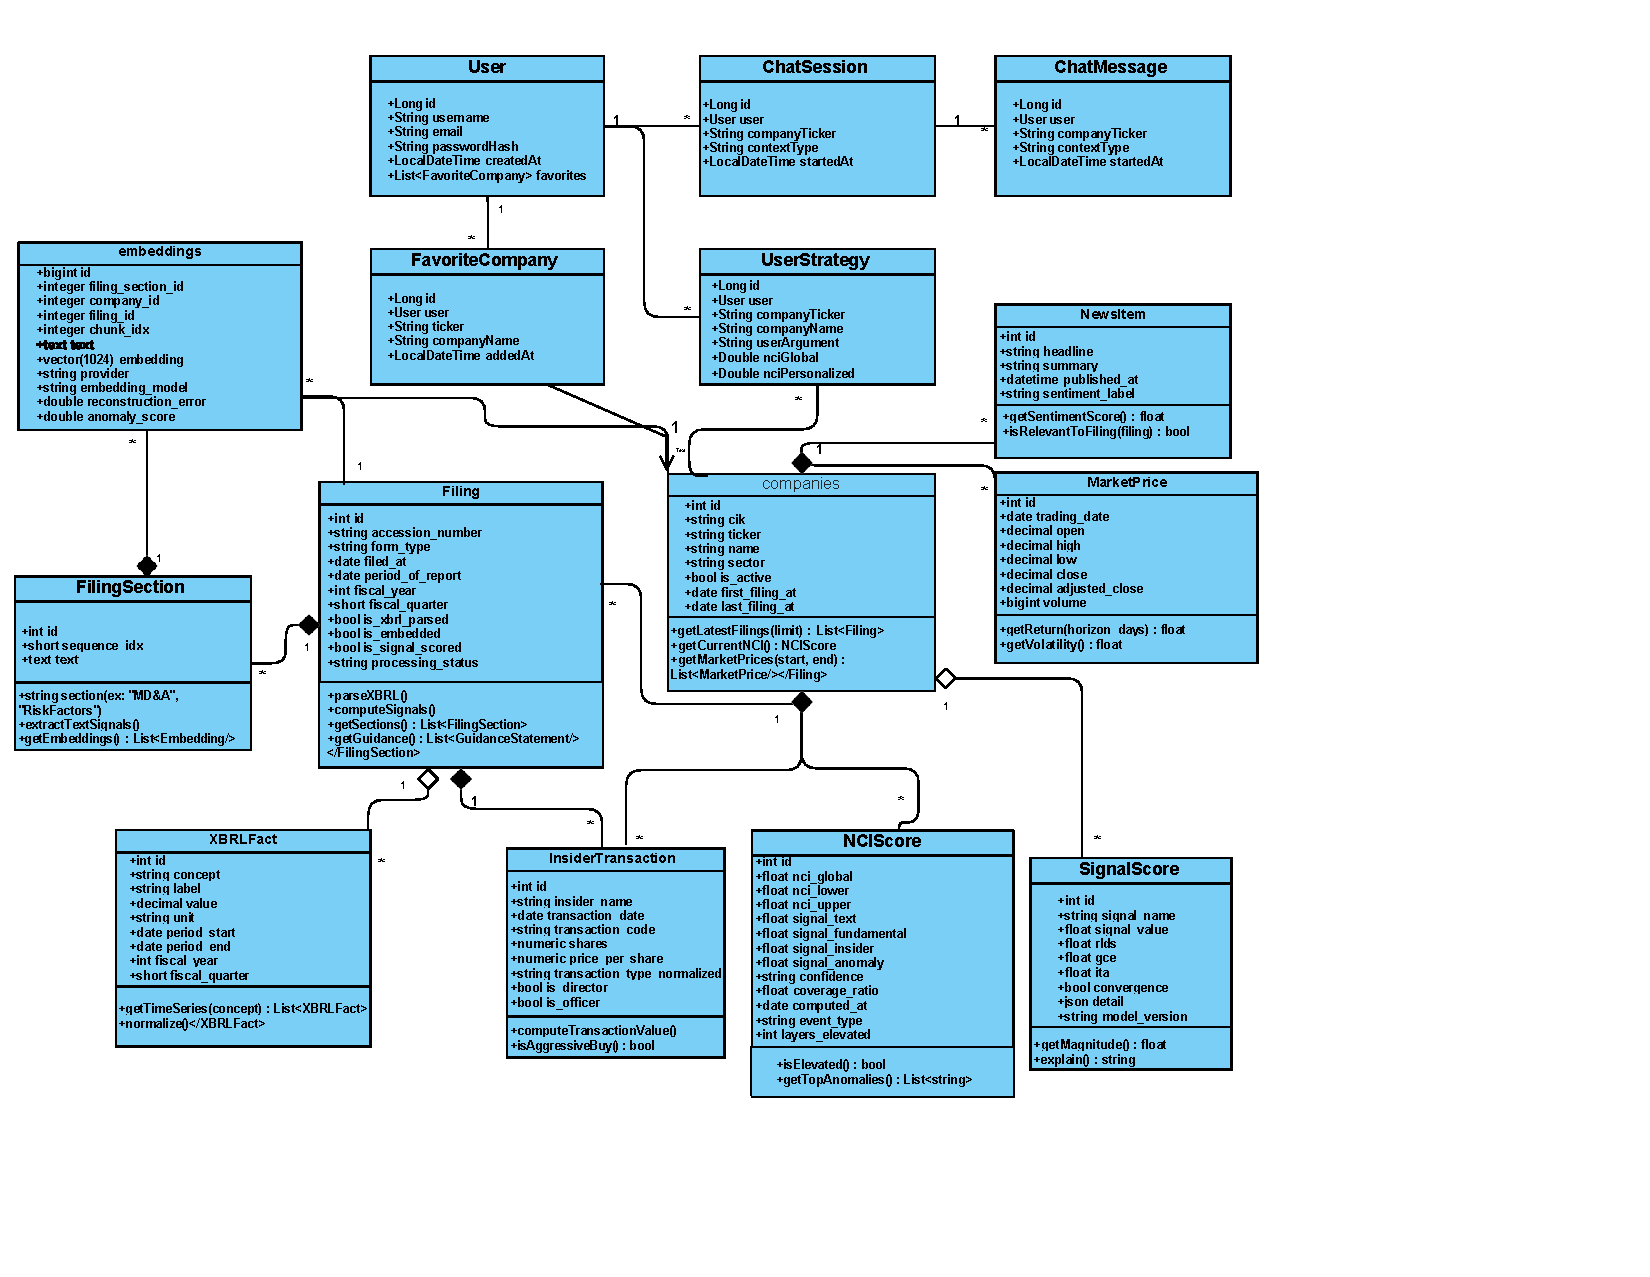
\includegraphics[width=1\textwidth]{images/FinPulse12.pdf}
    \caption{Diagramme de classes – Modèle de données et services}
    \label{fig:class}
\end{figure}
\newpage
\subsection{Diagrammes de séquences}
\subsubsection{Scénario : Inscription}
\subsubsection{Scénario : Connexion}
\subsubsection{Scénario : Consulter l'assistant ou générer une stratégie financière}
\begin{figure}[H]
    \centering
    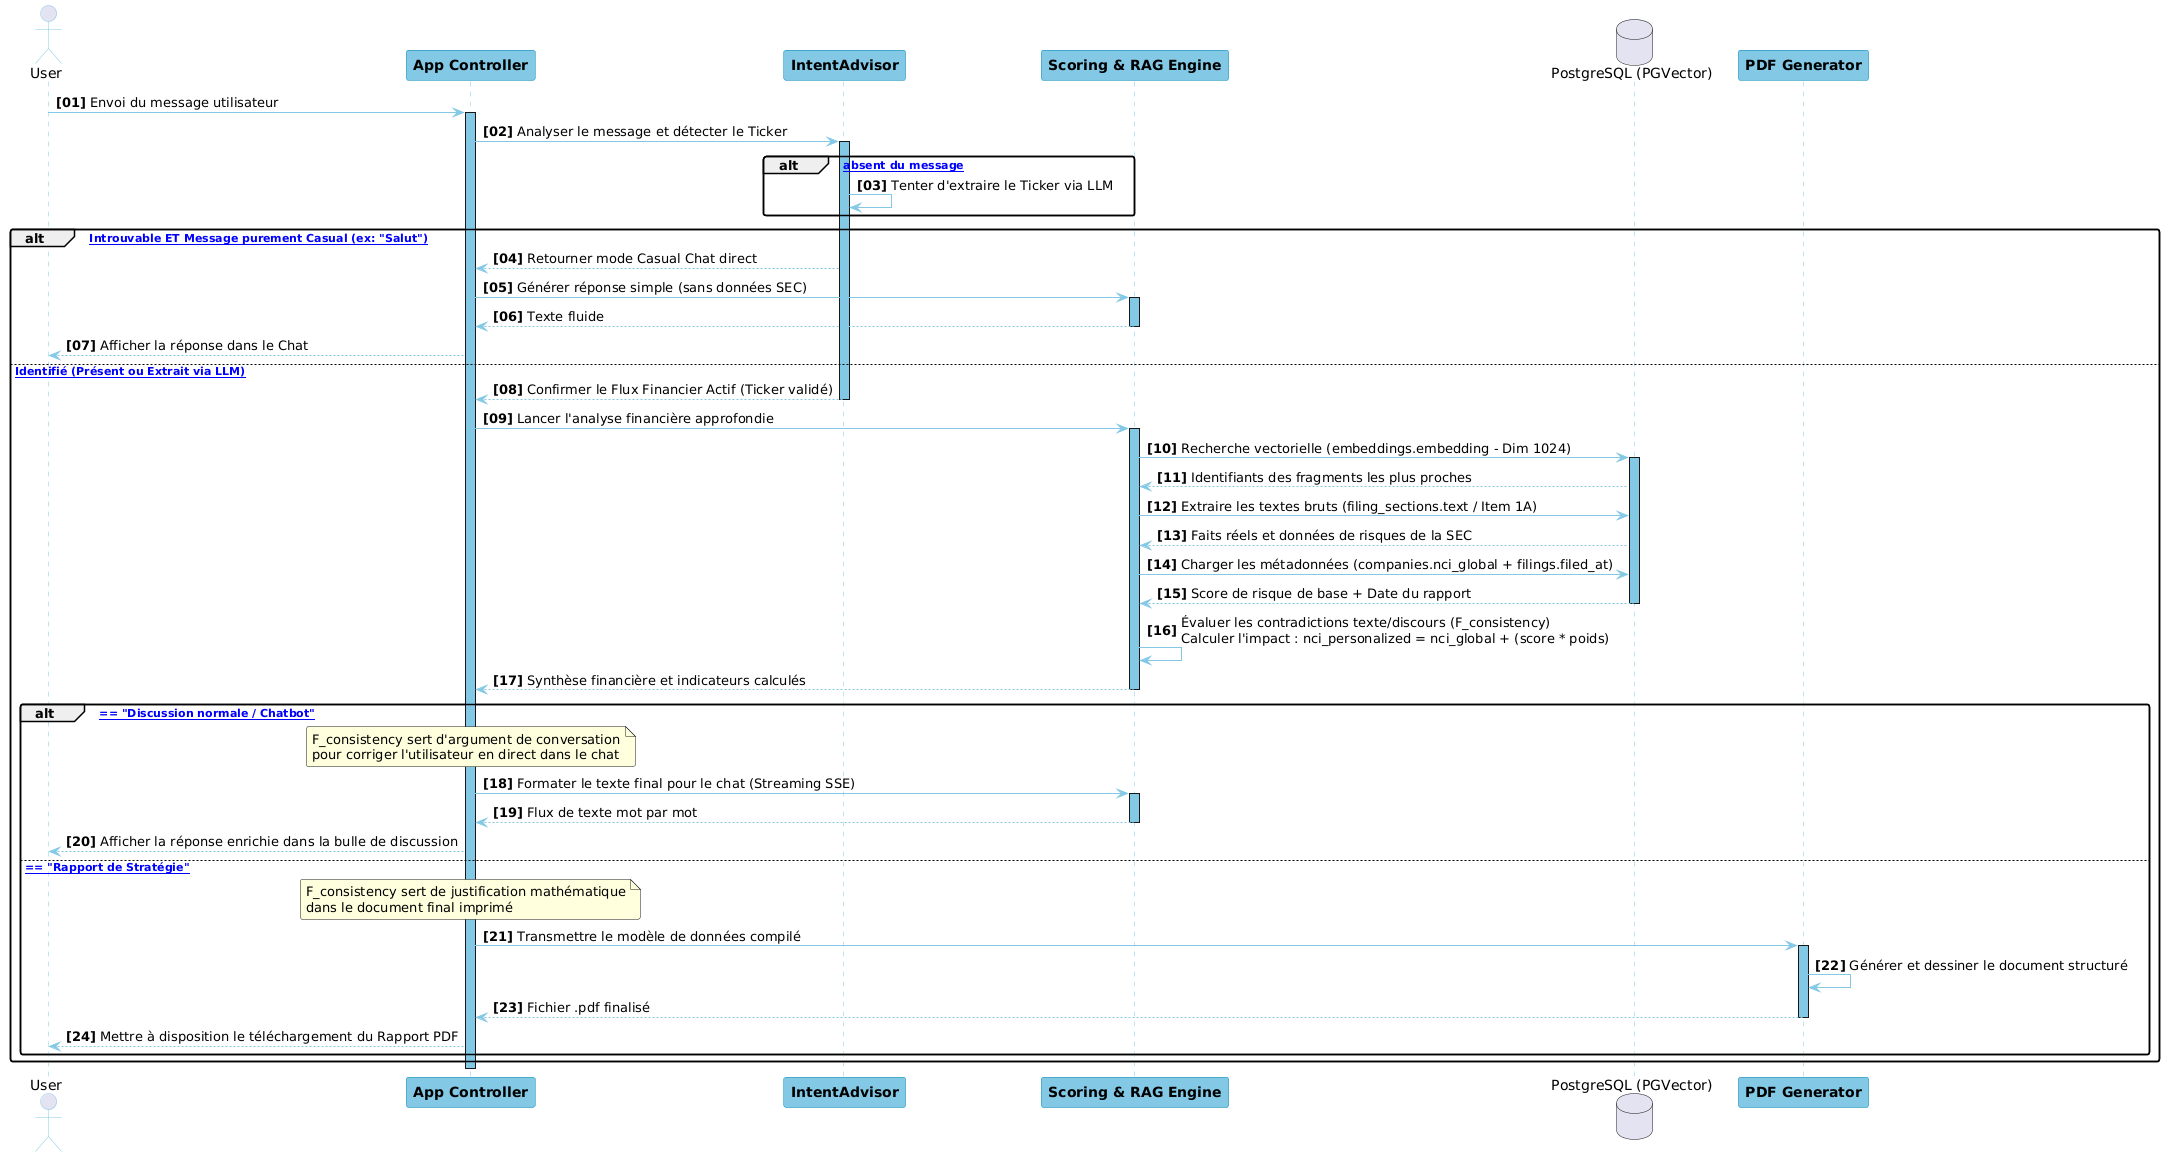
\includegraphics[width=1\linewidth]{images/sequenceeee.png}
    \caption{Scénario : Consulter l'assistant ou générer une stratégie financière}
    \label{fig:sequence-assistant-strategie}
\end{figure}
\section{Architecture logicielle}
FinPulse repose sur une architecture logicielle moderne conçue pour répondre aux exigences d’une plateforme d’analyse financière intelligente. Cette architecture vise à assurer une séparation claire des responsabilités entre les différents composants, tout en garantissant la performance, la sécurité et la scalabilité du système. Elle s’appuie sur une organisation en couches ainsi que sur une approche orientée services, permettant d’intégrer efficacement les modules d’intelligence artificielle, l’ingestion automatisée des données financières et l’interface utilisateur interactive. Cette conception facilite également la maintenance du système et l’évolution future de la plateforme par l’ajout de nouvelles sources de données ou de nouveaux agents d’analyse.
\subsection{Couches de l'architecture}
FinPulse repose sur une architecture à trois couches (Présentation, Application, Données) garantissant une séparation des responsabilités, une maintenabilité optimale et une scalabilité horizontale du système.
\subsubsection*{Couche Présentation:}
\begin{itemize}
    \item \textbf{Rôle} : La couche Présentation représente l’interface utilisateur de FinPulse. Elle assure l’interaction directe avec l’investisseur en offrant une navigation fluide et une visualisation claire des indicateurs financiers (NCI, sentiment, variations boursières, alertes, conversation avec l'assistant);
    \item \textbf{Responsabilités principales} :  Recherche et exploration des entreprises (Discover Page), Gestion des stratégies sauvegardées et monitoring,Gestion du profil utilisateur, Affichage dynamique des données;
    \item \textbf{Technologies utilisées} : Angular, CSS.
\end{itemize}

\subsubsection*{Couche Application:}
\begin{itemize}
    \item \textbf{Rôle} :  La couche application implémente la logique métier centralisée, l'orchestration des services et la gestion de l'authentification/autorisation. Elle constitue le cœur du système FinPulse.
    \item \textbf{Responsabilités principales} : Exposition des endpoints REST utilisés par Angular, Gestion de la Watchlist utilisateur (ajout/suppression d’entreprises), Orchestration du pipeline multi-agent , Traitement des requêtes utilisateur et dialogue conversationnel , Communication avec le service IA Python pour l’inférence deep learning et embeddings ,Gestion du caching avec Redis.

    \item \textbf{Technologies utilisées} : Spring Boot 3.4.5 (Spring Security , Spring Data , Spring AI), iText 7, WebFlux , Redis avec Spring Cache.

\end{itemize}
\subsubsection*{Couche  Données:}
\begin{itemize}
    \item \textbf{Rôle} :  La couche données gère l'ingestion, la transformation, le stockage et la récupération de toutes les données du système. Elle intègre deux composantes : le pipeline d'ingestion et la persistance.
    \item \textbf{Responsabilités principales} : Collecte de données auprès de cinq sources externes (SEC Edgar, FRED, données de marché, actualités, transactions insiders),  Normalisation et validation des données entrantes , Parsing XBRL et extraction de métriques financières structurées
    , Analyse de sentiment NLP (FinBERT) sur documents et actualités ,  Calcul des signaux de risque multi-couche (texte, numériques, comportementaux, marché, sentiment), Vectorisation de texte et stockage d'embeddings, Mise en cache distribuée et cache-aside pour performance .
    \item \textbf{Technologies utilisées} : Python , FastApi, PostgreSQL, PGVector, PyTorch 2.9, TensorFlow, Transformers 4.57, 

\end{itemize}
\subsection{Architecture système globale}
FinPulse intègre deux briques logicielles complémentaires en architecture microservices-like : un service backend Spring Boot (Multi-Agent-Assistant) qui gère l'interface utilisateur et l'orchestration métier, et un service Python (Data-Ingestion-Pipeline) qui gère l'ingestion et le traitement de données financières complexes. Ces deux services communiquent par REST API et partagent une infrastructure commune (PostgreSQL, Redis, Docker).
\subsubsection{Architecture Conceptuelle}
Le flux global suit le modèle suivant :

\begin{enumerate}
    \item L'utilisateur accède au Frontend Interface  et se connecte via /login (JWT).
    
    \item Après connexion, l'utilisateur utilise le Dashboard principal (Home Hub) pour :
    \begin{itemize}
        \item découvrir des entreprises
        \item gérer sa watchlist
        \item interagir avec l'AI Agent
        \item recevoir des alertes en temps réel
    \end{itemize}
    
    \item Le Frontend Interface envoie les actions utilisateur au Backend Spring Boot via REST API sécurisée par JWT.
    
    \item Le Backend gère :
    \begin{itemize}
        \item RAG SEC + SQL
        \item Orchestration multi-étapes
        \item 3 appels LLM (Mistral)
        \item streaming SSE pour la Watchlist et Notifications
    \end{itemize}
    
    \item Les données sont stockées dans la base (companies, embeddings, filings, chat\_sessions, chat\_messages, user\_strategies\ldots).
    
    \item En fonction de l'intention utilisateur :
    \begin{itemize}
        \item soit réponse Chatbot immédiate.
        \item soit création d'un rapport PDF complet pour une stratégie
    \end{itemize}
    
    \item Le Backend retourne au Frontend Interface :
    \begin{itemize}
        \item JSON (chat + scores + preuves + news)
        \item et si besoin PDF généré (download direct)
    \end{itemize}
\end{enumerate}
\subsubsection{Schéma de l'Architecture}
\begin{figure}[H]
    \centering
    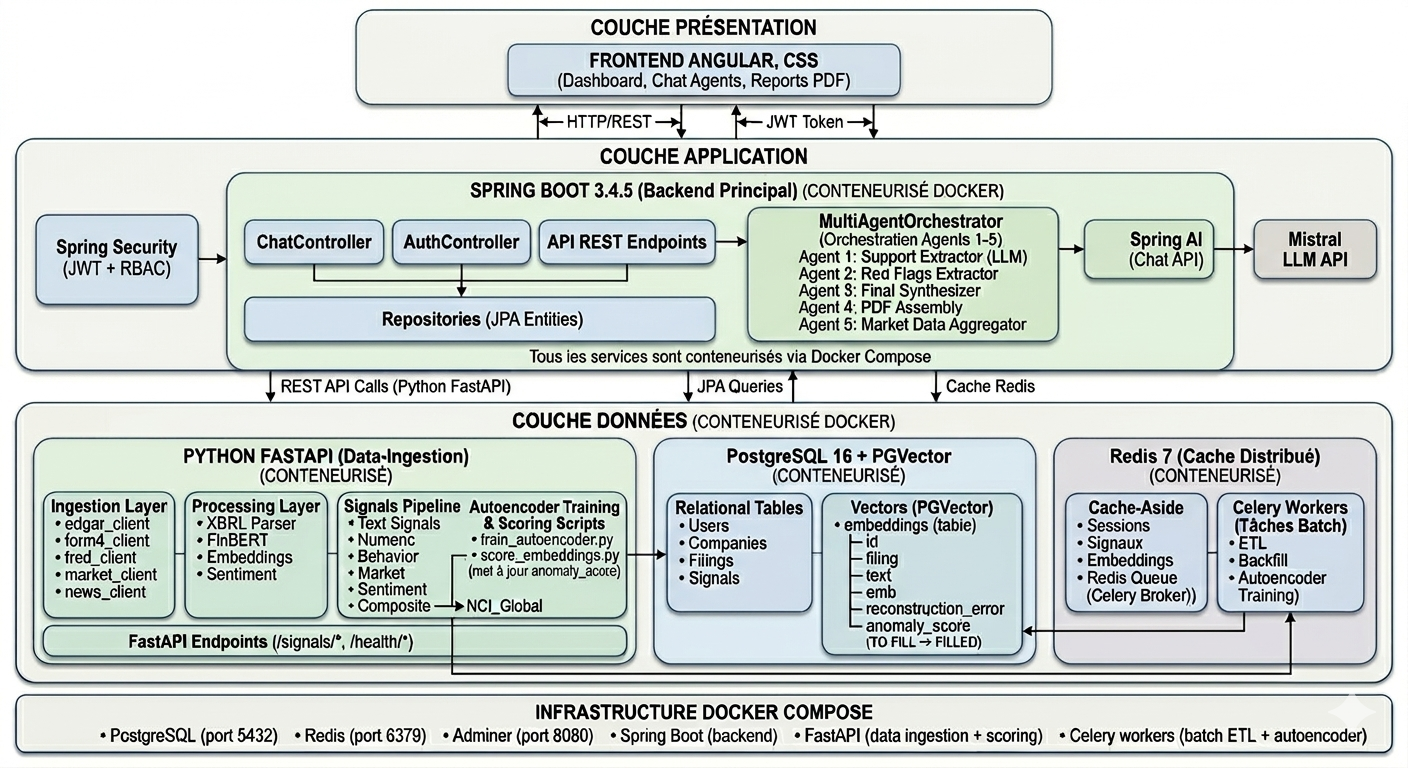
\includegraphics[width=1\linewidth]{images/thisoneeeee.png}
    \caption{Architecture FinPulse}
    \label{fig:architecture-finpulse}
\end{figure}

\subsection{Mécanisme de communication entre les couches }
\subsubsection{Communication Présentation $\leftrightarrow$ Application}
Le flux utilise le protocole \textbf{HTTP/REST} sécurisé par des \textbf{tokens JWT}. 
\begin{description}
    \item[Flux] : Angular transmet les requêtes via le header \textit{Authorization}. Le \textit{JwtAuthenticationFilter} de Spring Security valide l'accès avant traitement.
\end{description}
\subsubsection{Communication Inter-services (Spring Boot $\leftrightarrow$ Python)}
L'orchestrateur Spring Boot consomme les services de l'API FastAPI via \textbf{WebClient}.
\begin{description}
    \item [Résilience] : Implémentation du pattern \textit{Circuit Breaker} avec un timeout de 5s et des retries exponentiels.
\end{description}
\subsubsection{Gestion de la Persistance et du Cache}
\begin{itemize}
    \item \textbf{JPA/Hibernate} : Abstraction des requêtes SQL pour PostgreSQL.
    \item \textbf{Pattern Cache-Aside} : Utilisation de Redis pour réduire la latence sur les sessions et les scores NCI fréquents.
\end{itemize}
\subsection{Avantages de cette architecture }
\subsubsection{Modularité et Maintenabilité}
L'architecture en trois couches garantit une séparation claire des responsabilités. Chaque couche (Présentation, Application, Données) peut être développée, testée et maintenue indépendamment. Les deux services Python et Java sont découplés par des interfaces REST bien définies, permettant des évolutions indépendantes. Cette modularité réduit la complexité globale et facilite l'onboarding de nouveaux développeurs.
\subsubsection{Sécurité}
\begin{itemize}
    \item \textbf{JWT + Spring Security} : Authentification robuste et \textit{stateless}, assurant la gestion sécurisée des sessions et la protection des endpoints REST.
    
    \item \textbf{HTTPS/TLS} : Chiffrement du transport des données afin de garantir la confidentialité et l’intégrité des communications entre les clients et les services.
    
    \item \textbf{Isolation BD} : Cloisonnement des données utilisateurs via un filtrage systématique basé sur \texttt{userId}, empêchant tout accès non autorisé aux ressources d’autres utilisateurs.
    
    \item \textbf{Container Security} : Sécurisation des conteneurs Docker par scan des images, durcissement des configurations et gestion des secrets via des variables d’environnement.
\end{itemize}
\subsubsection{Performance et Résilience}
\begin{itemize}
    \item \textbf{Cache distribué Redis} : Réduction de la latence des requêtes fréquentes grâce au stockage en mémoire des données réutilisées (watchlist, scores NCI, résultats RAG).
    
    \item \textbf{Async Processing (Celery)} : Ingestion non-bloquante et traitement batch optimisé via des tâches asynchrones planifiées, améliorant la scalabilité du pipeline de données.
    
    \item \textbf{Connection Pooling} : PostgreSQL et Redis utilisent des pools de connexions afin d’éviter la saturation du serveur et d’optimiser la gestion des accès concurrents.
    
    \item \textbf{Circuit Breaker} : Les appels vers l’API Python sont protégés par un mécanisme de tolérance aux pannes avec fallback automatique, garantissant la continuité du service en cas d’indisponibilité.
    
    \item \textbf{Monitoring} : Spring Boot Actuator expose les métriques système et applicatives via l’endpoint \texttt{/actuator/metrics}, permettant le suivi des performances et la détection proactive des anomalies.
\end{itemize}
\subsubsection{Séparation des Responsabilités}
- Data-Ingestion-Pipeline : Pure data processing et IA (ETL, signaux, embeddings)\\
- Multi-Agent-Assistant : Pure business logic et orchestration agents LLM
- Chaque service excelle dans son domaine sans dupliquer la logique métier
\subsubsection{Extensibilité}
L'architecture multi-agent et composable permet l'ajout facile de nouveaux agents (Agent 6, 7, ...) sans impacter les existants. La couche signaux supporte l'intégration de nouvelles sources de données ou nouveaux types de signaux (behavioral, textual, etc.) par simple ajout de modules dans le pipeline.

\section{Conclusion}

Ce chapitre a permis de définir la conception fonctionnelle et technique de la plateforme \textbf{FinPulse}. Les contraintes du projet, les besoins fonctionnels et non fonctionnels ainsi que la modélisation UML ont été analysés afin de structurer une solution cohérente et adaptée aux exigences de performance, de sécurité et d’évolutivité.

L’architecture proposée constitue ainsi une base solide et stable pour assurer une implémentation maîtrisée du système. \\Sur cette base, la suite du travail consistera à concrétiser cette conception à travers la mise en œuvre effective de la solution.

